\documentclass{beamer}
\usepackage{tcolorbox}
\usepackage{hyperref}
\usepackage{booktabs}
\usepackage{siunitx}
\usepackage{tikz}
\usepackage{forest}
\usetikzlibrary{positioning}
\newdimen\nodeDist
\nodeDist=33mm
\usepackage{pgfplots}
\pgfplotsset{width=6cm,compat=1.9}

\usepgfplotslibrary{colorbrewer}



\usepackage{notation} % Custom package

%\beamerdefaultoverlayspecification{<+->}
% \newcommand{\data}{\mathcal{D}}
% \newcommand\Item[1][]{%
% 	\ifx\relax#1\relax  \item \else \item[#1] \fi
% 	\abovedisplayskip=0pt\abovedisplayshortskip=0pt~\vspace*{-\baselineskip}}

\graphicspath{ {imgs/} }

\usetheme{metropolis}           % Use metropolis theme


\title{Decision Trees}
\date{\today}
\author{Nipun Batra and teaching staff}
\institute{IIT Gandhinagar}

\begin{document}
	\maketitle
	
	
	
	\renewcommand{\arraystretch}{0.9}
	\begin{frame}{Training Data}
	\begin{tabular}{lllll||l} \toprule
	\textbf{Day} & \textbf{Outlook}  & \textbf{Temp} & \textbf{Humidity} & \textbf{Windy}  & \textbf{Play} \\ \midrule
	D1  & Sunny    & Hot  & High     & Weak   & No   \\
	D2  & Sunny    & Hot  & High     & Strong & No   \\
	D3  & Overcast & Hot  & High     & Weak   & Yes  \\
	D4  & Rain     & Mild & High     & Weak   & Yes  \\
	D5  & Rain     & Cool & Normal   & Weak   & Yes  \\
	D6  & Rain     & Cool & Normal   & Strong & No   \\
	D7  & Overcast & Cool & Normal   & Strong & Yes  \\
	D8  & Sunny    & Mild & High     & Weak   & No   \\
	D9  & Sunny    & Cool & Normal   & Weak   & Yes  \\
	D10 & Rain     & Mild & Normal   & Weak   & Yes  \\
	D11 & Sunny    & Mild & Normal   & Strong & Yes  \\
	D12 & Overcast & Mild & High     & Strong & Yes  \\
	D13 & Overcast & Hot  & Normal   & Weak   & Yes  \\
	D14 & Rain     & Mild & High     & Strong & No  \\ \bottomrule
	\end{tabular}
\end{frame}



\begin{frame}{Learnt Decision Tree}

\begin{tikzpicture}[
node/.style={%
	draw,
	rectangle,
},
]

\node [node] (A) {Outlook};
\path (A) ++(-150:\nodeDist) node [node] (B) {Humidity};
\path (A) ++(-90:\nodeDist/2) node [node, fill=green] (C) {Yes};
\path (A) ++(-30:\nodeDist) node [node] (D) {Wind};
\path (B) ++(-135:\nodeDist) node [node, fill=red] (E) {No};
\path (B) ++(-45:\nodeDist) node [node, fill=green] (F) {Yes};
\path (D) ++(-45:\nodeDist) node [node, fill=red] (G) {No};
\path (D) ++(-135:\nodeDist) node [node, fill=green] (H) {Yes};

\draw (A) -- (B) node [left,pos=0.25] {Sunny}(A);
\draw (A) -- (C) node [right,pos=0.8] {Overcast}(A);
\draw (A) -- (D) node [right,pos=0.5] {Rain}(A);
\draw (B) -- (E) node [left,pos=0.25] {High}(A);
\draw (B) -- (F) node [right,pos=0.25] {Normal}(C);
\draw (D) -- (G) node [right,pos=0.25] {Strong}(A);
\draw (D) -- (H) node [left,pos=0.25] {Weak}(A);
\end{tikzpicture}

\end{frame}

%\begin{frame}
%\begin{forest}
%	for tree={grow'=south}
%	[Outlook
%	[Humidity, edge label={node[midway,fill=gray,font=\scriptsize]{Sunny}} []]
%	[Wind, edge label={node[midway,fill=white,font=\scriptsize]{Rain}} [] [] []]
%	[Yes, edge label={node[midway,fill=white,font=\scriptsize]{Overcast}}]
%	]
%\end{forest}
%\end{frame}

\begin{frame}{Entropy}
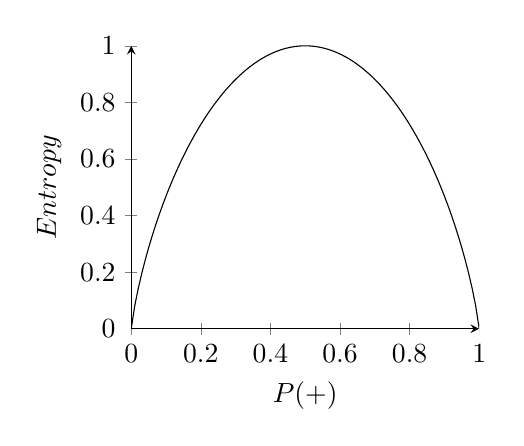
\begin{tikzpicture}
\begin{axis}[
axis lines = left,
xlabel = $P(+)$,
ylabel = {$Entropy$},
]
%Below the red parabola is defined
\addplot [
domain=0:1, 
samples=100, 
color=black
]
{-x*log2(x)-(1-x)*log2(1-x)};


\end{axis}
\end{tikzpicture}
\end{frame}
	
	
\begin{frame}{Information Gain}
$$
\operatorname{Gain}(S, A) \equiv \text { Entropy }(S)-\sum_{v \in V a l u e s(A)} \frac{\left|S_{v}\right|}{|S|} \text {Entropy}\left(S_{v}\right)
$$
\end{frame}
\begin{frame}{Learnt Decision Tree}
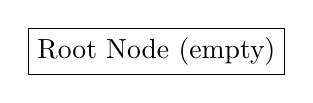
\begin{tikzpicture}[
node/.style={%
	draw,
	rectangle,
},
]

\node [node] (A) {Root Node (empty)};

\end{tikzpicture}

\end{frame}


\begin{frame}{Entropy calculated}
We have 14 examples in $S$: 5 No, 9 Yes

$$\operatorname{Entropy(S)} = -\operatorname{p}_{No}\operatorname{log_2}{\operatorname{p}_{No}}
-\operatorname{p}_{Yes}\operatorname{log_2}{\operatorname{p}_{Yes}}$$
$$
=-(5 / 14) \log _{2}(5 / 14)-(9 / 14) \log _{2}(9 / 14) =0.94
$$
\end{frame}

\begin{frame}{Information Gain for Outlook}
\begin{tabular}{l|l} \toprule
\textbf{Outlook} & \textbf{Play} \\ \midrule
Sunny    & No   \\
Sunny    & No   \\
Overcast & Yes  \\
Rain     & Yes  \\
Rain     & Yes  \\
Rain     & No   \\
Overcast & Yes  \\
Sunny    & No   \\
Sunny    & Yes  \\
Rain     & Yes  \\
Sunny    & Yes  \\
Overcast & Yes  \\
Overcast & Yes  \\
Rain     & No  \\ \bottomrule
\end{tabular}
\end{frame}

\begin{frame}{Information Gain for Outlook}
\begin{columns}


\begin{column}{.32\textwidth}
	\begin{table}
\begin{tabular}{l|l} \toprule
	\textbf{Outlook} & \textbf{Play} \\ \midrule
	Sunny    & No   \\
	Sunny    & No   \\
	Sunny    & No   \\
	Sunny    & Yes  \\
	Sunny    & Yes  \\

\bottomrule
\end{tabular}
We have 2 Yes, 3 No
Entropy = (-3/5)$\log_{2}$(-3/5) - (-2/5)$\log_{2}$(-2/5) = 0.971
\end{table}
\end{column}

\pause \begin{column}{.32\textwidth}
	\begin{table}


\begin{tabular}{l|l} \toprule
	\textbf{Outlook} & \textbf{Play} \\ \midrule

	Overcast & Yes  \\
	Overcast & Yes  \\
	Overcast & Yes  \\
	Overcast & Yes  \\ \bottomrule

\end{tabular}
We have 4 Yes, 0 No
Entropy = 0


	\end{table}


\end{column}


\pause \begin{column}{.32\textwidth}
	\begin{table}
\begin{tabular}{l|l} \toprule
	\textbf{Outlook} & \textbf{Play} \\ \midrule
	Rain     & Yes  \\
	Rain     & Yes  \\
	Rain     & No   \\
	Rain     & Yes  \\
	Rain     & No  \\ \bottomrule
\end{tabular}
We have 3 Yes, 2 No
Entropy = (-3/5)$\log_{2}$(-3/5) - (-2/5)$\log_{2}$(-2/5) = 0.971
\end{table}
\end{column}
\end{columns}
\end{frame}

\begin{frame}{Information Gain}
$$
\operatorname{Gain}(S, Outlook) = \text { Entropy }(S)-\sum_{v \in \{Rain, Sunny, Windy\}} \frac{\left|S_{v}\right|}{|S|} \text {Entropy}\left(S_{v}\right) 
$$

Gain (S, Outlook) $=$ Entropy $(\mathrm{S})$ -$(5 / 14)$* Entropy(S\textsubscript{Sunny})- $(4 / 14)$* Entropy (S\textsubscript{overcast})$-(5 / 14)$* Entropy(S\textsubscript{Rain}) \\

= 0.940 - 0.347 - 0.347 \\
= 0.246

\end{frame}

\begin{frame}

	
	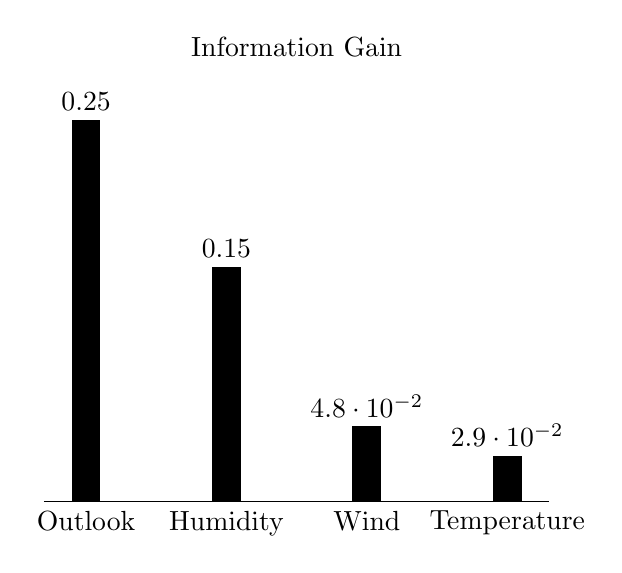
\begin{tikzpicture}
	\begin{axis}[
	symbolic x coords={Outlook,Humidity,Wind,Temperature},
	xtick=data,xtick pos=left, width=8cm,
	ytick pos=left,axis x line*=bottom,nodes near coords,hide y axis,title=Information Gain, ymin=0.0]
	\addplot[ybar,fill=black] coordinates {
		(Outlook,0.246)
		(Humidity,0.151)
		(Wind,0.048)
		(Temperature,0.029)
	};
	\end{axis}
	\end{tikzpicture}
	

\end{frame}
\textit{
\begin{frame}
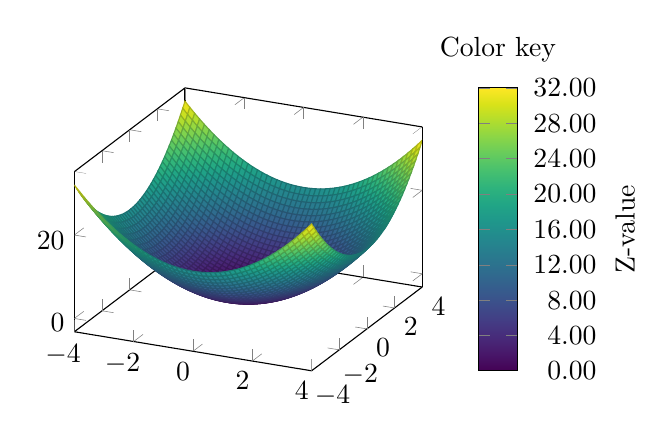
\begin{tikzpicture}
\begin{axis}[
domain=-4:4,
samples=50,
colormap/viridis,
colorbar,
colorbar style={
	title=Color key,
	ylabel=Z-value,
	ytick={0, 4, ..., 32},
	yticklabel style={
		text width=2.5em,
		align=right,
		/pgf/number format/.cd,
		fixed,
		fixed zerofill
	}
}
]
\addplot3 [surf] {x^2 + y^2};
\end{axis}
\end{tikzpicture}
\end{frame}}

\begin{frame}
\begin{tikzpicture}
\begin{axis}
[
title={Contour plot, view from top},
view={0}{90},
unit vector ratio*=1 1 1,
]
\addplot3[
contour gnuplot={levels={0.8, 0.4, 0.2, -0.2}}, samples=100,
]
{x^2+y^2};
\end{axis}
\end{tikzpicture}
\end{frame}

\begin{frame}
\begin{columns}[T] % align columns
	\begin{column}{.48\textwidth}
		\color{red}\rule{\linewidth}{4pt}
		
		Left Part
	\end{column}%
	\hfill%
	\begin{column}{.48\textwidth}
		\color{blue}\rule{\linewidth}{4pt}
		
		Right Part
	\end{column}%
\end{columns}
\end{frame}
\end{document}

\end{frame}

\begin{frame}{Example 1}
Let us consider the dataset given below
\begin{center}
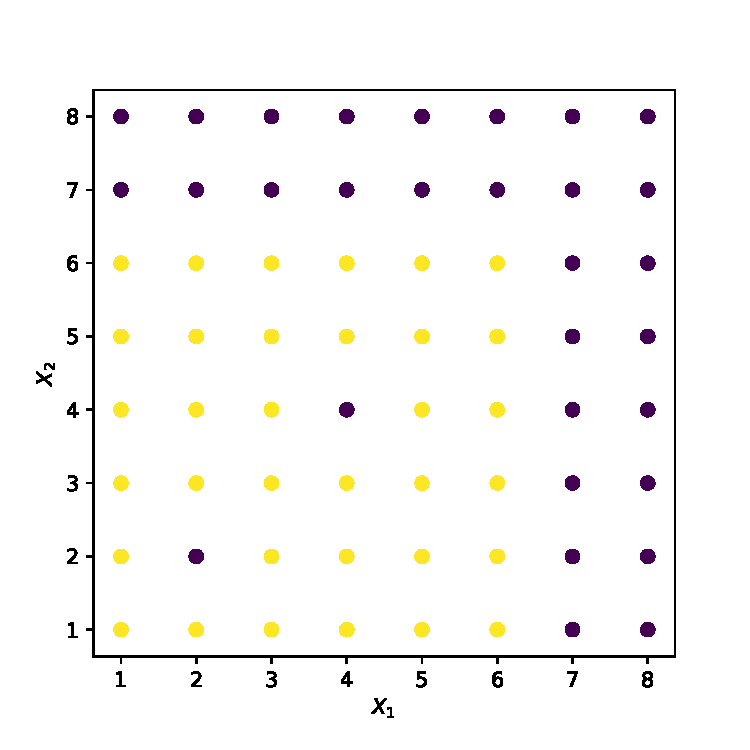
\includegraphics[scale=0.5]{dataset}
\end{center}
\end{frame}

\begin{frame}{Example 1}
What would be the prediction for decision tree with depth 0?
\begin{center}
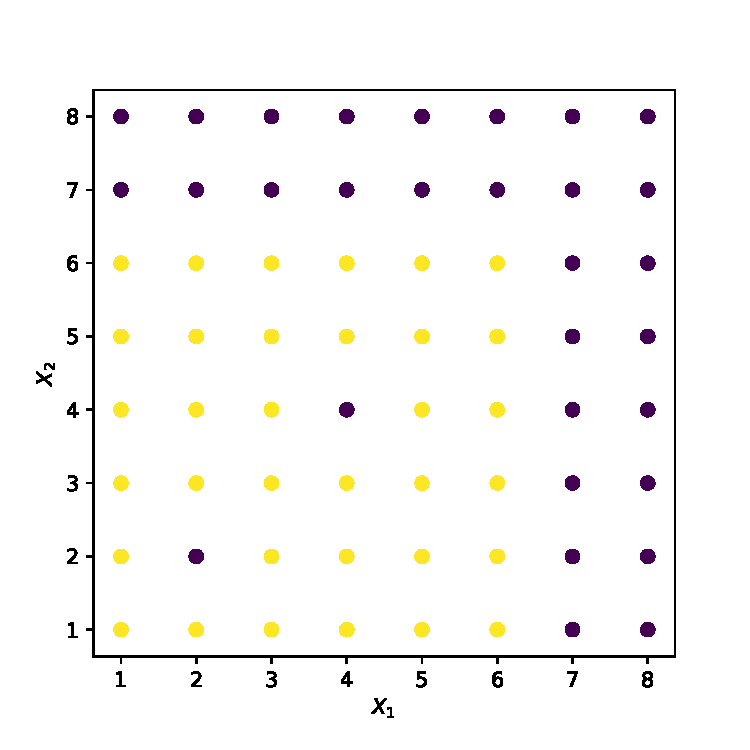
\includegraphics[scale=0.5]{dataset}
\end{center}
\end{frame}

\begin{frame}{Example 1}
Prediction for decision tree with depth 0.\\
Horizontal dashed line shows the predicted $Y$ value. It is the average of $Y$ values of all datapoints.\\
\begin{center}
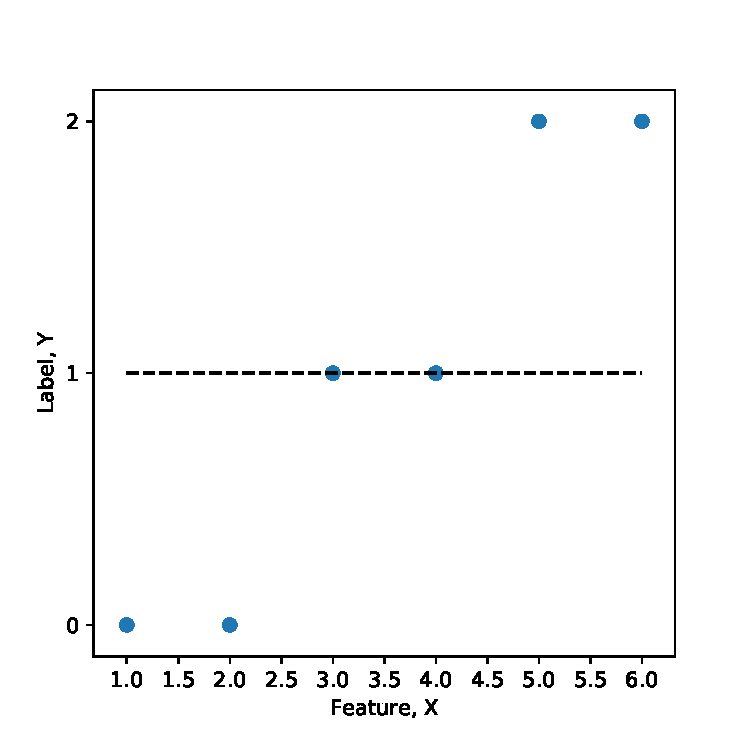
\includegraphics[scale=0.5]{depth-0-boundary}	
\end{center}
\end{frame}


\begin{frame}{Example 1}
What would be the decision tree with depth 1?
\begin{center}
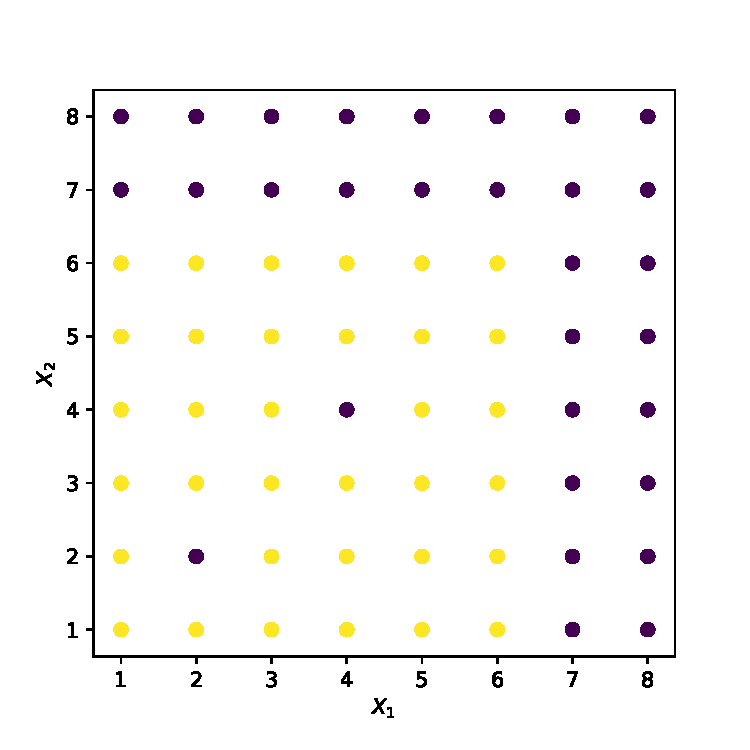
\includegraphics[scale=0.5]{dataset}
\end{center}
\end{frame}

\begin{frame}{Example 1}
Decision tree with depth 1
\begin{center}
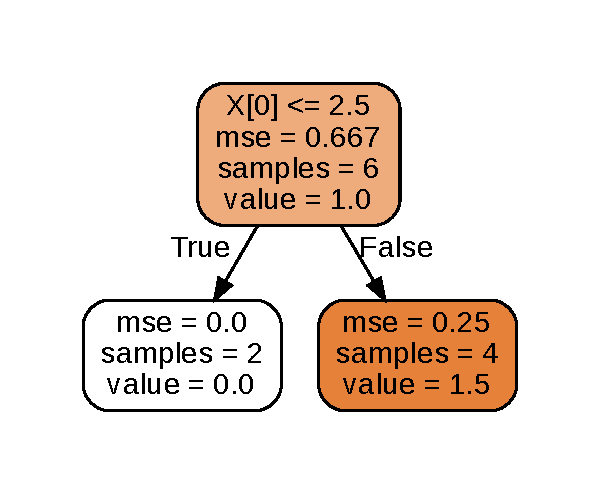
\includegraphics[scale=1]{depth-1-decision-tree}	
\end{center}
\end{frame}

\begin{frame}{Example 1}
The Decision Boundary
\begin{center}
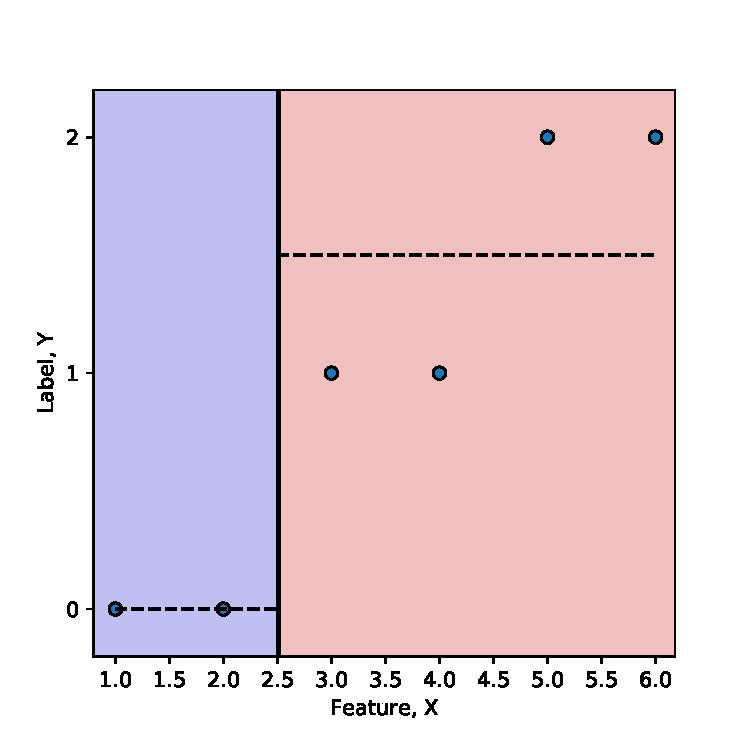
\includegraphics[scale=0.5]{depth-1-tree}
\end{center}
\end{frame}


\begin{frame}{Example 1}
What would be the decision tree with depth 2	?
\begin{center}
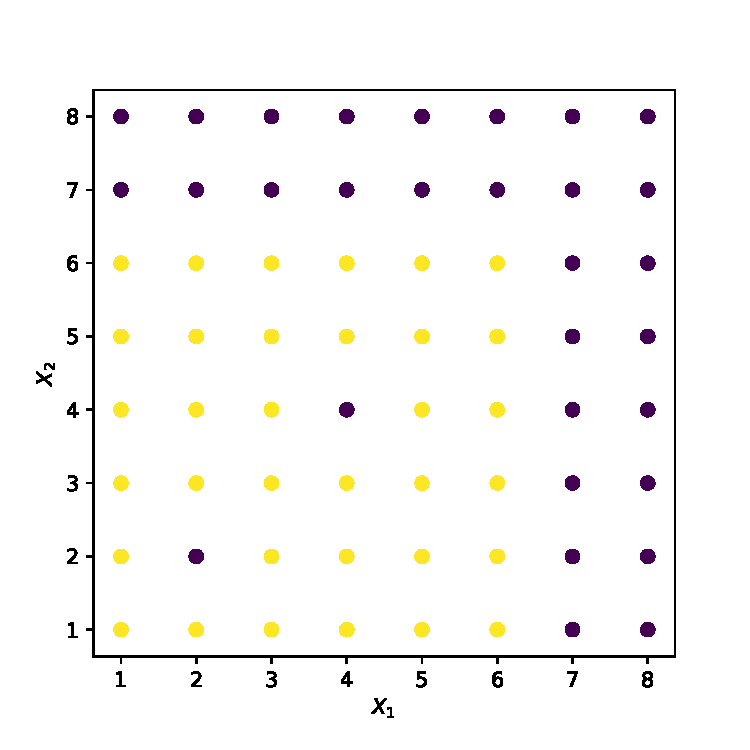
\includegraphics[scale=0.5]{dataset}
\end{center}
\end{frame}

\begin{frame}{Example 1}
Decision tree with depth 2
\begin{center}
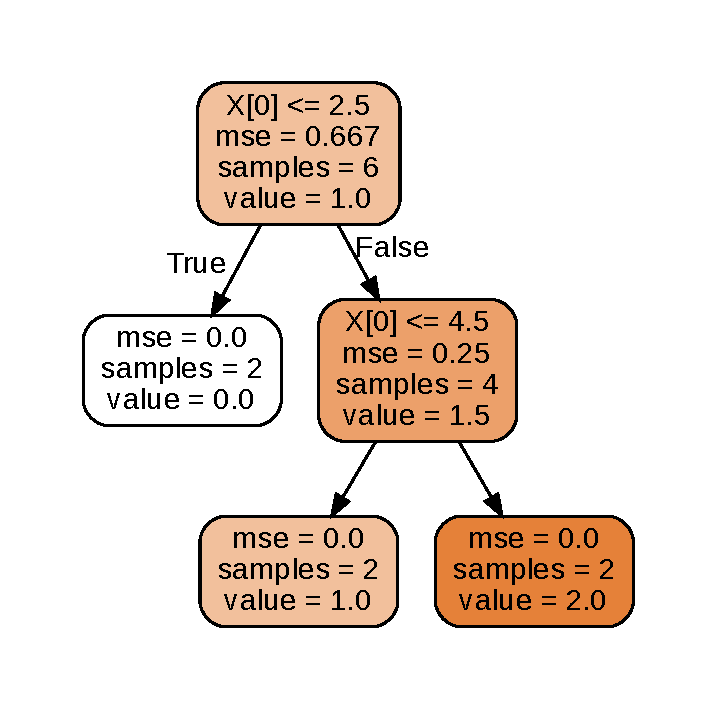
\includegraphics[scale=0.65]{depth-2-decision-tree}	
\end{center}
\end{frame}

\begin{frame}{Example 1}
The Decision Boundary
\begin{center}
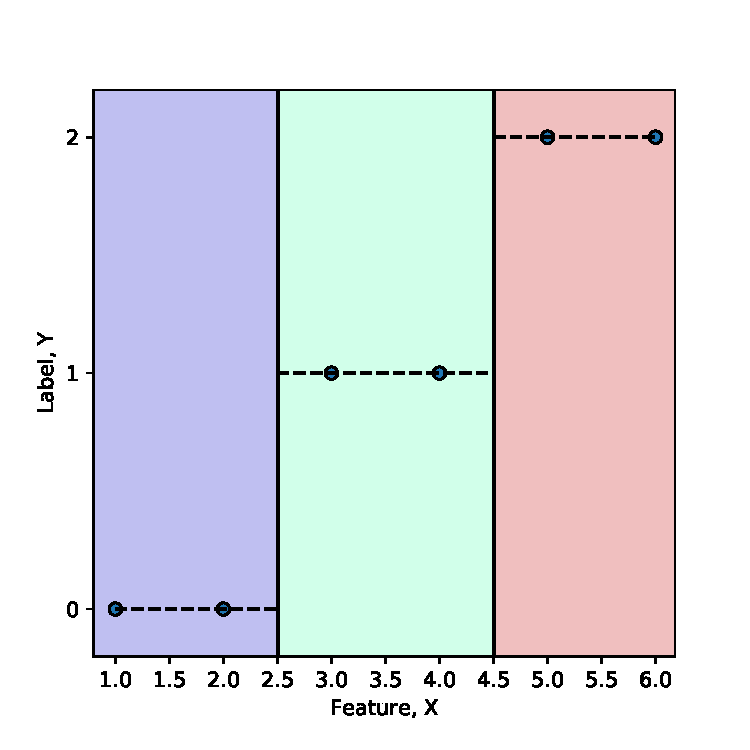
\includegraphics[scale=0.5]{depth-2-tree}
\end{center}
\end{frame}

\begin{frame}{Loss function}
\only<1-4>{
Here,  Feature is denoted by X and Label by Y.\\
Let the ``decision boundary'' or ``split" be at X = S.\\
Let the region X $<$ S, be region R$_1$.\\
Let the region X $>$ S, be region R$_2$.\\
\vspace{1cm}
}
\only<2-4>{
Then, let \\
$C_1$ = Mean ($Y_i | X_i \in R_1$) \\
$C_2$ = Mean ($Y_i | X_i \in R_2$) \\
}
\only<3-4>{
Loss = $\sum\limits_i$(($Y_i - C_1 | X_i \in R_1$)$^2 $ +  ($Y_i - C_2 | X_i \in R_2$)$^2 $)\\
\vspace{1cm}
}
\only<4>{
Our objective is to minimize the loss and find\\
$min_S $ $\sum\limits_i\left((Y_i - C_1 | X_i \in R_1)^2  +  (Y_i - C_2 | X_i \in R_2)^2 \right)$
}
\end{frame}

\begin{frame}{How to find optimal split ``S"?}
\end{frame}


\begin{frame}{How to find optimal split ``S"?}
\begin{enumerate}
\only<1-2>{
\item Sort all datapoints (X,Y) in increasing order of X.
\vspace{0.5cm}
}
\only<2>{
\item Evaluate the loss function for all\\
\vspace{0.25cm}
\begin{center}
$S = \frac{X_i + X_{i+1}}{2}$\\
\end{center}
\vspace{0.25cm}
and the select the S with minimum loss.
}
\end{enumerate} 
\end{frame}

\begin{frame}{A Question!}
Draw a regression tree for Y = sin(X), $0 \leq X \leq 2\pi$ 
\end{frame}

\begin{frame}{A Question!}
Dataset of Y = sin(X), $0 \leq X \leq 7$ with 10,000 points 
\begin{center}
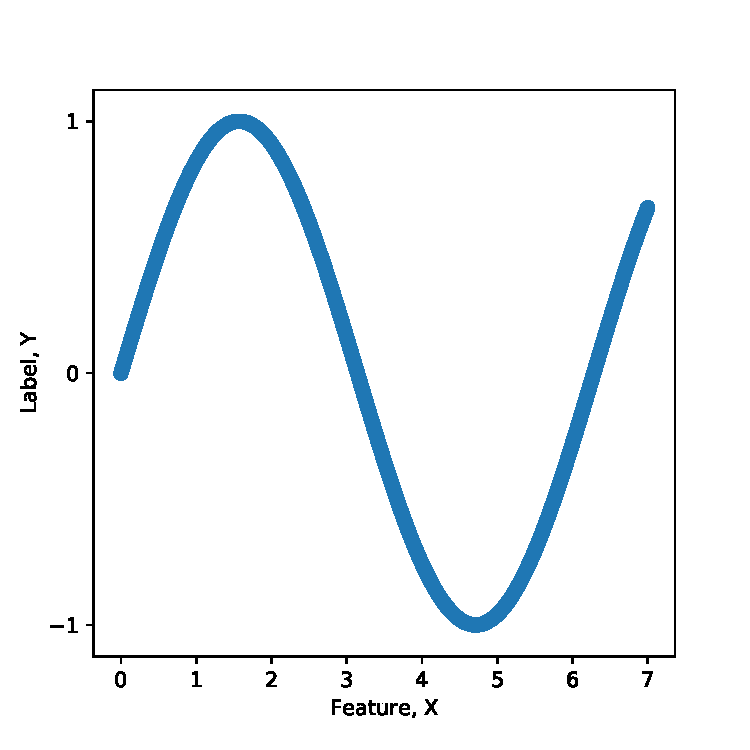
\includegraphics[scale=0.5]{sine-dataset}
\end{center}
\end{frame}

\begin{frame}{A Question!}
Regression tree of depth 1
\begin{center}
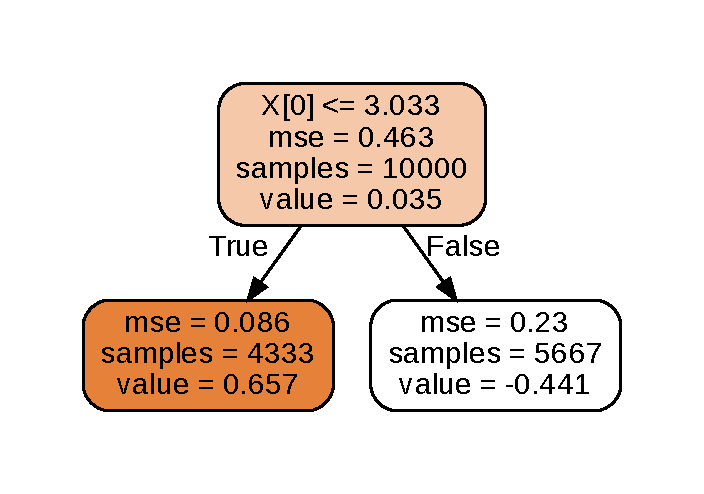
\includegraphics[scale=0.5]{sine-depth-1-decision-tree}
\end{center}
\end{frame}

\begin{frame}{A Question!}
Decision Boundary
\begin{center}
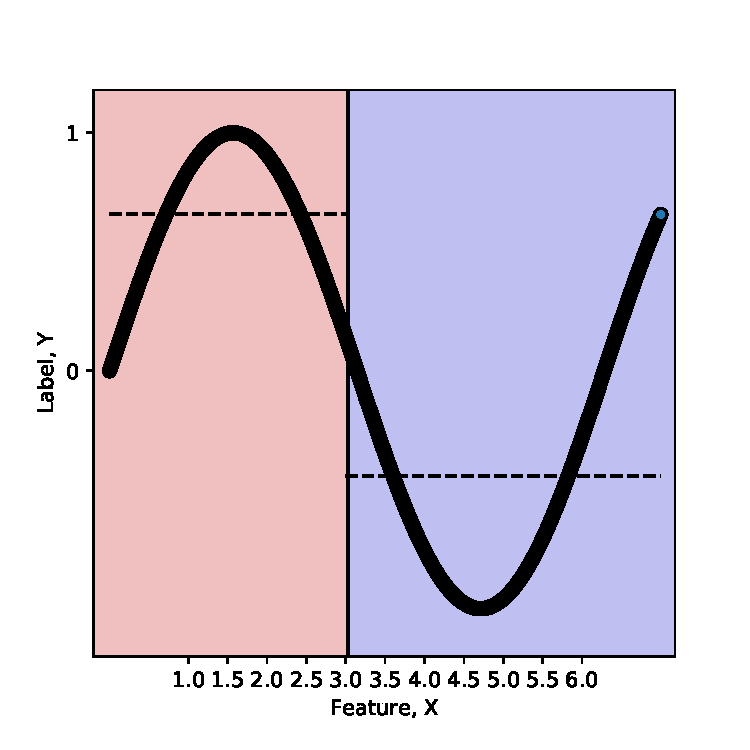
\includegraphics[scale=0.5]{sine-depth-1-tree}
\end{center}
\end{frame}

\begin{frame}{A Question!}
Regression tree with no depth limit is too big to fit in a slide. \\
It has of depth 20. The decision boundaries are in figure below.\\
\begin{center}
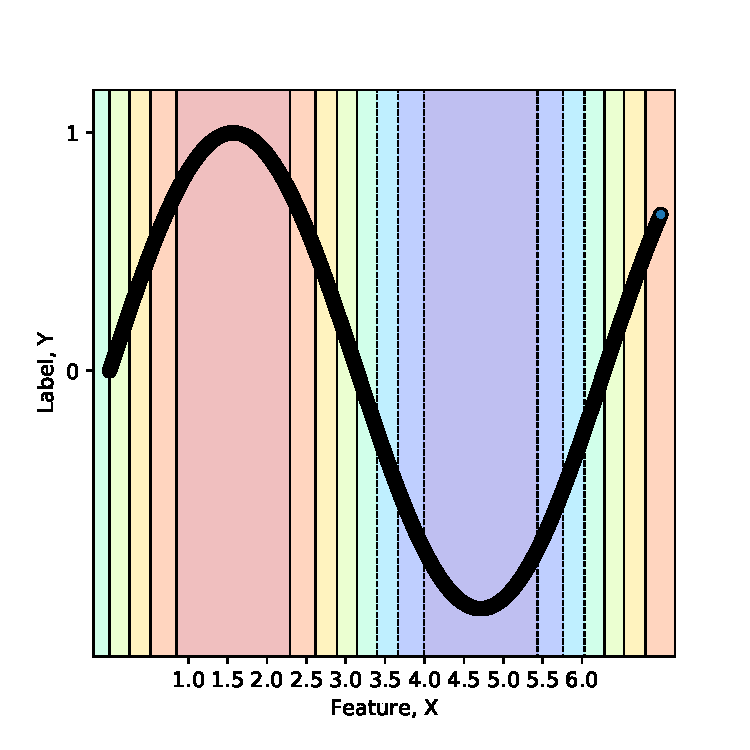
\includegraphics[scale=0.5]{sine-no-depth-tree}
\end{center}
\end{frame}

\begin{frame}{Code for examples}
\begin{center}
\href{https://colab.research.google.com/drive/1NnuVxypYfEOvpMbFHE4075CI-EkT8S7B}{Google Colab}
\end{center}
\end{frame}

\end{document}